
\input{./preamble.tex}

%%% Begin document
\begin{document}

\title{
	%\vspace{-1in}
	\usefont{OT1}{bch}{b}{n}
	\normalfont \normalsize \textsc{Instituto Tecnológico de Buenos Aires} \\ [25pt]
	\horrule{2pt} \\[0.4cm]
	\huge Assignment $N^o 2$ \\
	\horrule{2pt} \\[0cm]
\author{Group 2:\\Díaz Ian Cruz\\Lin Benjamín\\ Müller Malena\\Oh Victor \\ \\ Professors:\\Dewald Kevin\\Wundes Pablo Enrique\\ \\}
\text{Electrónica 3 - 2018}
}
\date{\today} %ver si dejar la de today o poner fecha fija que sea August 2018
\pagenumbering{arabic}

\maketitle
\newpage

% The \input command appends the content of the file directly into the document.
%\input{./preamble.tex}

%%% Begin document
\begin{document}

\input{./preamble.tex}

\begin{document}

%\begin{titlepage}
    
\newcommand{\HRule}{\rule{\linewidth}{0.5mm}} % Defines a new command for the horizontal lines, change thickness here
    
\center % Center everything on the page
     
%----------------------------------------------------------------------------------------
%	HEADING SECTIONS
%----------------------------------------------------------------------------------------
    
\textsc{\LARGE Instituto Tecnológico de Buenos Aires}\\[2cm] % Name of your university/college
\textsc{\Large Electronica III}\\[1.5cm] % Major heading such as course name
\textsc{\large Trabajo Práctico N° 2}\\[0.5cm] % Minor heading such as course title
    
%----------------------------------------------------------------------------------------
%	TITLE SECTION
%----------------------------------------------------------------------------------------
    
\HRule \\[0.5cm]
{ \huge \bfseries Trabajo Práctico de Laboratorio Nr. 2}\\[0.4cm] % Title of your document
\HRule \\[2cm]
     
%----------------------------------------------------------------------------------------
%	AUTHOR SECTION
%----------------------------------------------------------------------------------------
    
\begin{minipage}{0.4\textwidth}
\begin{flushleft} \large
\emph{Grupo 2:}\\		%names
[.3cm]
Victor \textsc{Oh}\\
Leg. ???\\ 
[.3cm]
Ian \textsc{Diaz}\\
Leg. ???\\ 
[.3cm]
Benjamín Carlos \textsc{Lin}\\
Leg. 57242 \\ 
[.3cm]
Malena \textsc{Muller}\\
Leg. ???\\ 
[.3cm]
\end{flushleft}
\end{minipage}
~
\begin{minipage}{0.4\textwidth}
\begin{flushright} \large
%\emph{Profesor:} \\
%[.3cm]
%Pablo  \textsc{Cossutta}\\ % Supervisor's Name
%Alejandra \textsc{Weill} \\% Supervisor's Name
%Matías  \textsc{Salvati} % Supervisor's Name
\end{flushright}
\end{minipage}\\[2cm]
    
%----------------------------------------------------------------------------------------
%	DATE SECTION
%----------------------------------------------------------------------------------------
    
\vfill
{\large Entregado: 17 de Octubre de 2018}\\[2cm]
    
\vfill 
    
\end{titlepage}
%
%\pagenumbering{roman}
%\tableofcontents
%\newpage
%\pagenumbering{arabic}
%
%Test Text

\section{\color{olive}Exercise 1: }

\subsection{\color{purple}Mealy State Machine}

In the Mealy state machine, the output value not only depends on the state we are but also depends on the input values. This is to say the output could be represented as a function like $Z=f(X_1.....X_n,Q_1....Q_n)$ where Z: output, Q: State and X:Input event as could be visualize:

 \begin{figure}[h!]
        \centering
        \includegraphics[scale=0.75]{Mealydiagram.png}
        \caption{\color{cyan}Mealy sate machine simple representation}
        \label{fig:ej1mealyr}
    \end{figure}

In this exercise, two sensors I and S function as input event to the state machine. Analyzing the possible states and event we obtain the following Mealy machine diagram:

 \begin{figure}[h!]
        \centering
        \includegraphics[scale=0.65]{ej1mealy.png}
        \caption{\color{cyan}Exercise 1: Mealy sate machine flow chart}
        \label{fig:ej1mealyd}
    \end{figure}

Which is represented as follow:

% Please add the following required packages to your document preamble:
% \usepackage{multirow}
\begin{table}[h!]
\centering
\begin{tabular}{|c|c|c|c|c|c|c|c|c|c|c|}
\hline
\multicolumn{3}{|c|}{\multirow{2}{*}{\textbf{State(Q)}}} & \multicolumn{8}{c|}{\textbf{Input(X)}} \\ \cline{4-11} 
\multicolumn{3}{|c|}{} & \multicolumn{2}{c|}{\textbf{I=0 S=0}} & \multicolumn{2}{c|}{\textbf{I=0 S=1}} & \multicolumn{2}{c|}{\textbf{I=1 S=0}} & \multicolumn{2}{c|}{\textbf{I=1 S=1}} \\ \hline
\textbf{Representation} & \textbf{Q2} & \textbf{Q1} & \textbf{Q2} & \textbf{Q1} & \textbf{Q2} & \textbf{Q1} & \textbf{Q2} & \textbf{Q1} & \textbf{Q2} & \textbf{Q1} \\ \hline
\textbf{Empty} & 0 & 0 & 0 & 0 & 0 & 1 & 1 & 0 & 1 & 1 \\ \hline
\textbf{Error} & 0 & 1 & 0 & 0 & 0 & 1 & 1 & 0 & 1 & 1 \\ \hline
\textbf{Half} & 1 & 0 & 0 & 0 & 0 & 1 & 1 & 0 & 1 & 1 \\ \hline
\textbf{Full} & 1 & 1 & 0 & 0 & 0 & 1 & 1 & 0 & 1 & 1 \\ \hline
\textbf{Output(Z)} & \textbf{Z1} & \textbf{Z2} & \textbf{0} & \textbf{0} & \textbf{1} & \textbf{1} & \textbf{1} & \textbf{0} & \textbf{1} & \textbf{1} \\ \hline
\end{tabular}
\caption{\color{cyan}Exercise 1: Mealy sate machine}
\end{table}

\pagebreak
So the logic circuit would be:

 \begin{figure}[h!]
        \centering
        \includegraphics[scale=1]{ej1mealycircuit.png}
        \caption{\color{cyan}Exercise 1: Mealy logic circuit}
        \label{fig:ej1mealyld}
    \end{figure}

We can notice that the input event and the output event are the same which could make the $Z_N=X_N$ with N: the output or input number, but as mention be in the Mealy state machine the output $Z=f(X_1.....X_n,Q_1....Q_n)$, so we considered essential the use of sate in the circuit is dependent with the state and the input to have a clear view of being a Mealy state machine.

\subsubsection{\color{Orange}Simulation}

For the simulation of this stage machine, as the pump B1 and B2 alternate their function when $I = 1 y S = 0$ and for the activation of the pump that depends on output voltage is needed the following circuit is added:

 \begin{figure}[h!]
        \centering
        \includegraphics[scale=1]{ej1mealycircuitplus.png}
        \caption{\color{cyan}Exercise 1: Mealy additional logic circuit for the simulation}
        \label{fig:ej1mealylp}
    \end{figure}
    
Simulation the complete circuit in Verilog and testing the possibles values of input in Gtkwave the result was:

 \begin{figure}[h!]
        \centering
        \includegraphics[scale=0.7]{ej1mealysim1.png}\\
        \vspace{0.2cm}
        \includegraphics[scale=0.73]{ej1mealysim2.png}
        \caption{\color{cyan}Exercise 1: Simulation results}
        \label{fig:ej1mealyw}
    \end{figure}

%%%%%%%%%%%%%%%%%%%%%%%%%%%%%%%%%%%%%%%%
%Para Maleeeee
\pagebreak
Esto es Y1
\begin{center}
        \begin{Karnaugh}
            %cada 4 es una fila, la col 3 es la 4ta columna y 3fila es la 4 fila
            \contingut{
            0,0,1,0,
            0,X,X,X,
            1,0,0,0,
            0,X,X,X}
            \implicant{2}{6}{red}
            \implicant{8}{8}{green}
%            \implicant{12}{8}{orange}
%            \implicantdaltbaix[3pt]{1}{9}{blue}
            %\implicantcantons[2pt]{orange}
            %\implicantcostats{4}{14}{green}
        \end{Karnaugh}
    \end{center}

Y2
\begin{center}
        \begin{Karnaugh}
            %cada 4 es una fila, la col 3 es la 4ta columna y 3fila es la 4 fila
            \contingut{
            0,0,1,0,
            0,X,X,X,
            0,1,1,0,
            1,X,X,X}
            \implicant{2}{10}{red}
            \implicant{12}{14}{green}
%            \implicant{12}{8}{orange}
            \implicant{13}{9}{blue}
%            \implicantdaltbaix[3pt]{1}{9}{blue}
            %\implicantcantons[2pt]{orange}
            %\implicantcostats{4}{14}{green}
        \end{Karnaugh}
    \end{center}
  
  Y3  
\begin{center}
        \begin{Karnaugh}
            %cada 4 es una fila, la col 3 es la 4ta columna y 3fila es la 4 fila
            \contingut{
            0,0,0,0,
            0,X,X,X,
            0,0,0,1,
            0,X,X,X}
            \implicant{15}{11}{red}
%            \implicant{12}{14}{green}
%%            \implicant{12}{8}{orange}
%            \implicant{13}{9}{blue}
%            \implicantdaltbaix[3pt]{1}{9}{blue}
            %\implicantcantons[2pt]{orange}
            %\implicantcostats{4}{14}{green}
        \end{Karnaugh}
    \end{center}
    
    Z
    \begin{center}
        \begin{Karnaughvuit}
            %cada 4 es una fila, la col 3 es la 4ta columna y 3fila es la 4 fila
            \minterms{4}
        \maxterms{0,1,2,3}
        \indeterminats{5,6,7}
            \implicant{4}{6}{red}
%            \implicant{12}{14}{green}
%%            \implicant{12}{8}{orange}
%            \implicant{13}{9}{blue}
%            \implicantdaltbaix[3pt]{1}{9}{blue}
            %\implicantcantons[2pt]{orange}
            %\implicantcostats{4}{14}{green}
        \end{Karnaughvuit}
    \end{center}

%%%%%%%%%%%%%%%%%%%%%%%%%%%%%%%%%%%%%%%


\end{document}













\section{Moore's Finite State Machine}

Moore's Finite State Machine (FSM) follows a model where the next state of the machine is determined by the current
inputs and its current state, while the output is determined by the current state of the machine, following the
designed combinational logic.

\subsection{Design}

Given the specifications required of the pump controller, the functionality of the fsm was represented
on Figure \ref{fig:moore_flow} and on Table \ref{fig:moore_table}, where "LnA" stands for "Last not Activated".

\begin{figure}[h]
    \begin{center}
        \begin{tikzpicture}[node distance = 5cm, auto]
    %place nodes
    \node [block] (empty) {Empty B1:On B2:On};
    \node [decision, below of = empty] (toggle) {Last Not Activated Pump};
    \node [block, left of = toggle]  (only_one) {Half Full: B1:On B2:Off LnA=B2};
    \node [block, right of = toggle] (only_two) {Half Full: B1:Off B2:On LnA=B1};
    \node [block, below of = toggle] (full) {Full: B1:Off B2:Off};
    %place lines
    \path [line] (empty) -- node [near start] {I=1,S=0} (toggle);
    \path [line] (toggle) -- node [near start] {B1} (only_one);
    \path [line] (toggle) -- node [near start] {B2} (only_two);
    \path [line] (full) -- node [near start] {I=1,S=0} (toggle);
    \path [line] (only_one) |- node [near start] {I=1,S=1} (full);
    \path [line] (only_two) |- node [near start] {I=1,S=1} (full);
    \path [line] (only_one) |- node [near start] {I=0,S=0} (empty);
    \path [line] (only_two) |- node [near start] {I=0,S=0} (empty);

\end{tikzpicture}
        \caption{Flow Diagram for Moore's Machine}
        \label{fig:moore_flow}
    \end{center}
\end{figure}

\begin{table}[ht]
    \begin{center}
        \begin{tabular}{|c|c|c|c|c|c|c|}
    \hline
    \multirow{3}{*}{Current State} & \multicolumn{4}{c}{Next State} & \multicolumn{2}{|c|}{Output} \\
    & S I & S I & S I & S I & \multirow{2}{*}{B1} & \multirow{2}{*}{B2} \\
    & 0 0 & 0 1 & 1 0 & 1 1 & & \\
    \hline
    Empty (0 0) & Empty & Half Full & Error & Full & 1 & 1 \\
    Half Full (0 1)& Empty & Half Full & Error & Full & $\sim$LnA & LnA \\
    Error (1 0)& Empty & Half Full & Error & Full & 0 & 0 \\
    Full (1 1)& Empty & Half Full & Error & Full & 0 & 0 \\
    \hline
\end{tabular}
        \caption{State Transition Table}
        \label{fig:moore_table}
    \end{center}
\end{table}

It can be observed that an error state was added. This was to cover every possible case of inputs. It was decided that
in case a "strange" input was received (Superior sensor activated while the Inferior sensor is not), both pumps should
stop working, as that seemed to be the safer decision, as this seemed to simply be a replenishment system and an empty
tank would alert the user of the error.

After deducing the combinational logic behind the next state assignment and the corresponding outputs for each state,
and taking into consideration the available components in the laboratory, the circuit in Figure \ref{fig:moore_circuit}
was obtained.

\begin{figure}
    \begin{center}
        \includegraphics[width=\linewidth]{circuit.png}
        \caption{Resulting circuit logic diagram}
        \label{fig:moore_circuit}
    \end{center}
\end{figure}

\subsection{Simulation}

Before physically implementing the FSM, first it was simulated in Verilog and ran through a testbench, 
where the waveform in Figure \ref{fig:moore_gtk} was obtained with gtkwave.

\begin{figure}
    \begin{center}
        \includegraphics[width=\linewidth]{gtkwave.png}
        \caption{Simulation results from gtkwave}
        \label{fig:moore_gtk}
    \end{center}
\end{figure}

It needs to be mentioned that in the design, a method of resetting the machine was included in case it was needed.
This reset case will set the LnA variable to 0 (which arms B1 for use) and deactivate both pumps until it is no longer
set.

\subsection{Physical Implementation}

After confirming the correct behaviour of the device, it was implemented on a Printed Circuit Board with the schematic
on Figure \ref{fig:moore_schem}.

\begin{figure}[ht]
    \begin{center}
        \includegraphics[width=\linewidth]{schematic.png}
        \caption{Device Schematic}
        \label{fig:moore_schem}
    \end{center}
\end{figure}

\begin{figure}[ht]
    \begin{center}
        \includegraphics[scale=0.5]{final_build.png}
        \includegraphics[scale=0.85]{final_back.png}
        \caption{Final Physical device (front/back)}
        \label{fig:moore_build}
    \end{center}
\end{figure}

After it was fully implemented and tested, several measurements were taken to figure out its characteristics.
In Figures \ref{fig:moore_nres} and \ref{fig:moore_nres_delay} both the functionality and the delay between the output
and the reset input can be seen and were measured to be 6.6ns.

\begin{figure}[ht]
    \begin{center}
        \includegraphics[width=0.75\linewidth]{images/e3e1_1_4nreset.png}
        \caption{Reset (pink) functionality testing}
        \label{fig:moore_nres}
    \end{center}
\end{figure}

\begin{figure}[ht]
    \begin{center}
        \includegraphics[width=0.75\linewidth]{images/e3e1_nreset_delay.png}
        \caption{Reset (pink) delay measurements with B1(green) and B2(blue)}
        \label{fig:moore_nres_delay}
    \end{center}
\end{figure}

The delay between the clock's positive edge and the output signals was also measured to be around 30ns in Figure \ref{fig:moore_delays}.

\begin{figure}[ht]
    \begin{center}
        \includegraphics[width=0.75\linewidth]{images/e3e1_1.png}
        \includegraphics[width=0.75\linewidth]{images/e3e1_1k.png}
        \includegraphics[width=0.75\linewidth]{images/e3e1_100k_.png}
        \caption{I/O Delay measurements at 1Hz, 1 kHz and 100 kHz respectively}
        \label{fig:moore_delays}
    \end{center}
\end{figure}

Lastly, some general testing for the correct behaviour of the machine was tested, which was the one expected and
designed, as well as consistent to the one obtained in the Verilog simulation. From Figures \ref{fig:moore_max} and 
\ref{fig:moore_min} it can be seen that the maximum output voltage is around 4.3V when fed with a 5V source and a
minimum of near 0V, taking into account the noise.

\begin{figure}[ht]
    \begin{center}
        \includegraphics[width=0.75\linewidth]{images/e3e1_1s4i_2b1_2b2_v1.png}
        \caption{High I/O voltage measurements}
        \label{fig:moore_max}
    \end{center}
\end{figure}

\begin{figure}[ht]
    \begin{center}
        \includegraphics[width=0.75\linewidth]{images/e3e1_1s4i_2b1_2b2_v0.png}
        \caption{Low I/O voltage measurements}
        \label{fig:moore_min}
    \end{center}
\end{figure}

\newpage
\subsection{Conclusions}
From all the measurements taken from the physical device and the simulations ran in Verilog, it can be concluded
that, given the case use this device would have, it is working as expected, with low delays between input and
output signals and accounting for all possible input cases, with a safety precausion of disabling all pumps from
activating if there is an error in the system or it is wished to be shut down.


%\newpage
\pagenumbering{roman}
\section{Appendix}

\begin{figure}[h!] %cambio la H por!
\begin{centering}
\includegraphics[scale=0.4]{../E4TP1/images/5}
\par\end{centering}
\caption{\color{cyan}Verilog implementation of Excercise 4}
\label{fig:figura4.6}
\end{figure}

\begin{figure}[h!]%cambio la H por!
\begin{centering}
\includegraphics[scale=0.4]{../E4TP1/images/6}
\par\end{centering}
\caption{\color{cyan}Terminal's output of Excercise 4}
\label{fig:figura4.7}
\end{figure}


%%% End document
\end{document}
\input{./preamble.tex}

\begin{document}

%\begin{titlepage}
    
\newcommand{\HRule}{\rule{\linewidth}{0.5mm}} % Defines a new command for the horizontal lines, change thickness here
    
\center % Center everything on the page
     
%----------------------------------------------------------------------------------------
%	HEADING SECTIONS
%----------------------------------------------------------------------------------------
    
\textsc{\LARGE Instituto Tecnológico de Buenos Aires}\\[2cm] % Name of your university/college
\textsc{\Large Electronica III}\\[1.5cm] % Major heading such as course name
\textsc{\large Trabajo Práctico N° 2}\\[0.5cm] % Minor heading such as course title
    
%----------------------------------------------------------------------------------------
%	TITLE SECTION
%----------------------------------------------------------------------------------------
    
\HRule \\[0.5cm]
{ \huge \bfseries Trabajo Práctico de Laboratorio Nr. 2}\\[0.4cm] % Title of your document
\HRule \\[2cm]
     
%----------------------------------------------------------------------------------------
%	AUTHOR SECTION
%----------------------------------------------------------------------------------------
    
\begin{minipage}{0.4\textwidth}
\begin{flushleft} \large
\emph{Grupo 2:}\\		%names
[.3cm]
Victor \textsc{Oh}\\
Leg. ???\\ 
[.3cm]
Ian \textsc{Diaz}\\
Leg. ???\\ 
[.3cm]
Benjamín Carlos \textsc{Lin}\\
Leg. 57242 \\ 
[.3cm]
Malena \textsc{Muller}\\
Leg. ???\\ 
[.3cm]
\end{flushleft}
\end{minipage}
~
\begin{minipage}{0.4\textwidth}
\begin{flushright} \large
%\emph{Profesor:} \\
%[.3cm]
%Pablo  \textsc{Cossutta}\\ % Supervisor's Name
%Alejandra \textsc{Weill} \\% Supervisor's Name
%Matías  \textsc{Salvati} % Supervisor's Name
\end{flushright}
\end{minipage}\\[2cm]
    
%----------------------------------------------------------------------------------------
%	DATE SECTION
%----------------------------------------------------------------------------------------
    
\vfill
{\large Entregado: 17 de Octubre de 2018}\\[2cm]
    
\vfill 
    
\end{titlepage}
%
%\pagenumbering{roman}
%\tableofcontents
%\newpage
%\pagenumbering{arabic}
%
%Test Text

\section{\color{olive}Exercise 1: }

\subsection{\color{purple}Mealy State Machine}

In the Mealy state machine, the output value not only depends on the state we are but also depends on the input values. This is to say the output could be represented as a function like $Z=f(X_1.....X_n,Q_1....Q_n)$ where Z: output, Q: State and X:Input event as could be visualize:

 \begin{figure}[h!]
        \centering
        \includegraphics[scale=0.75]{Mealydiagram.png}
        \caption{\color{cyan}Mealy sate machine simple representation}
        \label{fig:ej1mealyr}
    \end{figure}

In this exercise, two sensors I and S function as input event to the state machine. Analyzing the possible states and event we obtain the following Mealy machine diagram:

 \begin{figure}[h!]
        \centering
        \includegraphics[scale=0.65]{ej1mealy.png}
        \caption{\color{cyan}Exercise 1: Mealy sate machine flow chart}
        \label{fig:ej1mealyd}
    \end{figure}

Which is represented as follow:

% Please add the following required packages to your document preamble:
% \usepackage{multirow}
\begin{table}[h!]
\centering
\begin{tabular}{|c|c|c|c|c|c|c|c|c|c|c|}
\hline
\multicolumn{3}{|c|}{\multirow{2}{*}{\textbf{State(Q)}}} & \multicolumn{8}{c|}{\textbf{Input(X)}} \\ \cline{4-11} 
\multicolumn{3}{|c|}{} & \multicolumn{2}{c|}{\textbf{I=0 S=0}} & \multicolumn{2}{c|}{\textbf{I=0 S=1}} & \multicolumn{2}{c|}{\textbf{I=1 S=0}} & \multicolumn{2}{c|}{\textbf{I=1 S=1}} \\ \hline
\textbf{Representation} & \textbf{Q2} & \textbf{Q1} & \textbf{Q2} & \textbf{Q1} & \textbf{Q2} & \textbf{Q1} & \textbf{Q2} & \textbf{Q1} & \textbf{Q2} & \textbf{Q1} \\ \hline
\textbf{Empty} & 0 & 0 & 0 & 0 & 0 & 1 & 1 & 0 & 1 & 1 \\ \hline
\textbf{Error} & 0 & 1 & 0 & 0 & 0 & 1 & 1 & 0 & 1 & 1 \\ \hline
\textbf{Half} & 1 & 0 & 0 & 0 & 0 & 1 & 1 & 0 & 1 & 1 \\ \hline
\textbf{Full} & 1 & 1 & 0 & 0 & 0 & 1 & 1 & 0 & 1 & 1 \\ \hline
\textbf{Output(Z)} & \textbf{Z1} & \textbf{Z2} & \textbf{0} & \textbf{0} & \textbf{1} & \textbf{1} & \textbf{1} & \textbf{0} & \textbf{1} & \textbf{1} \\ \hline
\end{tabular}
\caption{\color{cyan}Exercise 1: Mealy sate machine}
\end{table}

\pagebreak
So the logic circuit would be:

 \begin{figure}[h!]
        \centering
        \includegraphics[scale=1]{ej1mealycircuit.png}
        \caption{\color{cyan}Exercise 1: Mealy logic circuit}
        \label{fig:ej1mealyld}
    \end{figure}

We can notice that the input event and the output event are the same which could make the $Z_N=X_N$ with N: the output or input number, but as mention be in the Mealy state machine the output $Z=f(X_1.....X_n,Q_1....Q_n)$, so we considered essential the use of sate in the circuit is dependent with the state and the input to have a clear view of being a Mealy state machine.

\subsubsection{\color{Orange}Simulation}

For the simulation of this stage machine, as the pump B1 and B2 alternate their function when $I = 1 y S = 0$ and for the activation of the pump that depends on output voltage is needed the following circuit is added:

 \begin{figure}[h!]
        \centering
        \includegraphics[scale=1]{ej1mealycircuitplus.png}
        \caption{\color{cyan}Exercise 1: Mealy additional logic circuit for the simulation}
        \label{fig:ej1mealylp}
    \end{figure}
    
Simulation the complete circuit in Verilog and testing the possibles values of input in Gtkwave the result was:

 \begin{figure}[h!]
        \centering
        \includegraphics[scale=0.7]{ej1mealysim1.png}\\
        \vspace{0.2cm}
        \includegraphics[scale=0.73]{ej1mealysim2.png}
        \caption{\color{cyan}Exercise 1: Simulation results}
        \label{fig:ej1mealyw}
    \end{figure}

%%%%%%%%%%%%%%%%%%%%%%%%%%%%%%%%%%%%%%%%
%Para Maleeeee
\pagebreak
Esto es Y1
\begin{center}
        \begin{Karnaugh}
            %cada 4 es una fila, la col 3 es la 4ta columna y 3fila es la 4 fila
            \contingut{
            0,0,1,0,
            0,X,X,X,
            1,0,0,0,
            0,X,X,X}
            \implicant{2}{6}{red}
            \implicant{8}{8}{green}
%            \implicant{12}{8}{orange}
%            \implicantdaltbaix[3pt]{1}{9}{blue}
            %\implicantcantons[2pt]{orange}
            %\implicantcostats{4}{14}{green}
        \end{Karnaugh}
    \end{center}

Y2
\begin{center}
        \begin{Karnaugh}
            %cada 4 es una fila, la col 3 es la 4ta columna y 3fila es la 4 fila
            \contingut{
            0,0,1,0,
            0,X,X,X,
            0,1,1,0,
            1,X,X,X}
            \implicant{2}{10}{red}
            \implicant{12}{14}{green}
%            \implicant{12}{8}{orange}
            \implicant{13}{9}{blue}
%            \implicantdaltbaix[3pt]{1}{9}{blue}
            %\implicantcantons[2pt]{orange}
            %\implicantcostats{4}{14}{green}
        \end{Karnaugh}
    \end{center}
  
  Y3  
\begin{center}
        \begin{Karnaugh}
            %cada 4 es una fila, la col 3 es la 4ta columna y 3fila es la 4 fila
            \contingut{
            0,0,0,0,
            0,X,X,X,
            0,0,0,1,
            0,X,X,X}
            \implicant{15}{11}{red}
%            \implicant{12}{14}{green}
%%            \implicant{12}{8}{orange}
%            \implicant{13}{9}{blue}
%            \implicantdaltbaix[3pt]{1}{9}{blue}
            %\implicantcantons[2pt]{orange}
            %\implicantcostats{4}{14}{green}
        \end{Karnaugh}
    \end{center}
    
    Z
    \begin{center}
        \begin{Karnaughvuit}
            %cada 4 es una fila, la col 3 es la 4ta columna y 3fila es la 4 fila
            \minterms{4}
        \maxterms{0,1,2,3}
        \indeterminats{5,6,7}
            \implicant{4}{6}{red}
%            \implicant{12}{14}{green}
%%            \implicant{12}{8}{orange}
%            \implicant{13}{9}{blue}
%            \implicantdaltbaix[3pt]{1}{9}{blue}
            %\implicantcantons[2pt]{orange}
            %\implicantcostats{4}{14}{green}
        \end{Karnaughvuit}
    \end{center}

%%%%%%%%%%%%%%%%%%%%%%%%%%%%%%%%%%%%%%%


\end{document}














%EXCERCISE 2 :)

\section{\color{olive}Excercise 2: State Machines to Detect the sequence 1-1-0-1}
In this exercise, the detection of the sequence 1-1-0-1 inside a longer sequence of bits, is done with a Moore's state machine and with a Mealy's state machine. The main difference between these two state machines is that in Moore's one, the output only depends on the present state of the machine, while in Mealy's one, the output depends on the present state as well as on the input. This causes a time displacement between the output of both state machines. Moore's output "answers" to the input one clock later after having reached the new state, while Mealy's output "answers" immediatly during the same clock that the input arrives. This is because Mealy's reacts not only according to the present state, but also depending on the input's value.

For the implementation of both state machines, five states are needed and they are represented with the letters from A to E:\\ 
- A (000): "IDLE", the state in which the first digit of the sequence has not yet been detected.\\
- B (001): The first digit of the sequence, "1", has arrived.\\
- C (010): The second digit of the sequence, "1",  has arrived.\\
- D (011): The third digit of the sequence, "0", has arrived.\\
- E (100): The last digit of the sequence, "1", has arrived.\\ \\
The states are digitally represented with three bits, as they allow to get five different combinations, so that the name of each state is represented with a binary number. Such representation is the one givin between parenthese, after the name of each state.  It is important to mention that no matter which is the present state, whenever a "0" arrives from reset, the state changes to state A (IDLE). 

\subsection{\color{purple}Moore Type State Machine}

In figure % poner figura
it is represented the sequence detection with the Moore's state machine.

\begin{figure}[H]
\centering
\includegraphics[scale=0.5]{../Exercise2/EJ2MOORE}
\caption{\color{cyan}Moore's State Machine, for detecting the sequence 1-1-0-1.}
\label{MOOREFSM}
\end{figure}

From above's diagram (the one in figure FIGURA1), the following table \ref {measej1} is obtained. 
\begin{table}[H]
\begin{center}
\begin{tabular}{|c|c c c|c|}
\hline
Present State & & Next State & & Output z \\
 & w=0 & & w=1 &   \\
\hline
\hline
A & A & & B & 0   \\
\hline
B & A & & C & 0   \\
\hline
C & D & & C & 0   \\
\hline
D & A & & E & 0   \\
\hline
E & A & & C & 1   \\
\hline
\hline
\end{tabular}
\end{center}
\caption{\label{measej1}\color{cyan}Moore's Next States and Outputs.}
\end{table}

From the previous table \ref {measej1} the following Karnaugh maps are used to get to simple logic expressions.


\subsection{\color{purple}Mealy Type State Machine}

In figure \ref {MealyEFSM} it is represented the sequence detection with the Mealy's state machine.

\begin{figure}[H]
\centering
\includegraphics[scale=0.5]{../Exercise2/EJ2MEALY}
\caption{\color{cyan}Mealy's State Machine, for detecting the sequence 1-1-0-1.}
\label{MealyEFSM}
\end{figure}

It can be seen how in this case, the transition between one state to another now also causes a change in the output. It doesn't wait to get to the new state in order to change it. The following table is obtained from above's diagram in figure \ref {measej2} .
\begin{table}[H]
\begin{center}
\begin{tabular}{|c|c c c|c c c|}
\hline
Present State & & Next State & & & Output z & \\
 &  & & & & depending on w&  \\
 & w=0 & & w=1 & w=0& &w=1  \\
\hline
\hline
A & A & & B & 0 & & 0   \\
\hline
B & A & & C & 0 & & 0   \\
\hline
C & D & & C & 0 & & 0 \\
\hline
D & A & & E & 0 & & 1  \\
\hline
E & A & & C & 0 & & 0 \\
\hline
\hline
\end{tabular}
\end{center}
\caption{\label{measej2}\color{cyan}Mealy's Next States and Outputs.}
\end{table}



\section{\color{olive}Exercise 3}

For this exercise we were asked to implement the Moore machine shown
on Figure \ref{3_1}, but with one condition, everything inside our
machine should work on 3.3v and inputs and outputs should work on
5v logic.

\begin{figure}[H]
\begin{centering}
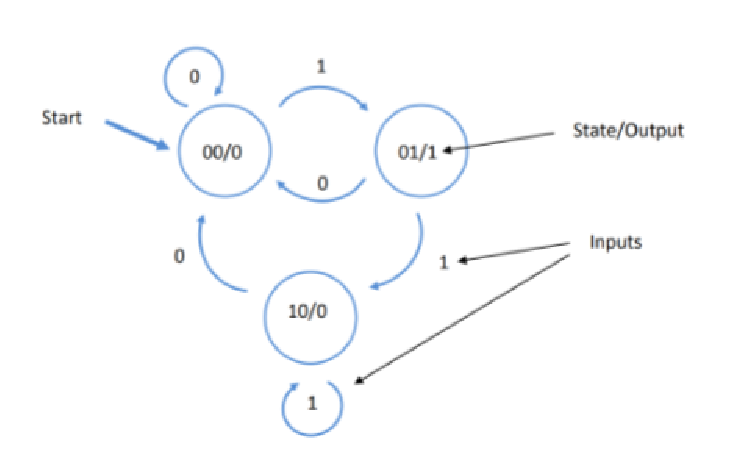
\includegraphics[scale=0.7]{../Exercise3/Assignment/images/Diagram}
\par\end{centering}
\caption{Moore Machine}
\label{3_1}
\end{figure}

\subsection{\color{purple}State Machine Implementation}

We proceeded to convert the diagram to a table that represents it,
and we got Table \ref{3_t_1}, and by transforming each bit (Output,
and next states bits) into a truth table, we could create our logic
implementation for each bit. The Truth Tables are shown on Tables
\ref{3_t_2}.

\begin{table}[H]
\begin{centering}
\begin{tabular}{|c|c|c|c|}
\hline 
State & W=0 & W=1 & Output\tabularnewline
\hline 
\hline 
00 & 00 & 01 & 0\tabularnewline
\hline 
01 & 00 & 10 & 1\tabularnewline
\hline 
10 & 00 & 10 & 0\tabularnewline
\hline 
\end{tabular}
\par\end{centering}
\caption{Moore Machine Table}
\label{3_t_1}

\end{table}

\begin{table}[H]
\begin{centering}
\begin{tabular}{|c|c|}
\hline 
S1 S0 & Output\tabularnewline
\hline 
\hline 
00 & 0\tabularnewline
\hline 
01 & 1\tabularnewline
\hline 
10 & 0\tabularnewline
\hline 
11 & x\tabularnewline
\hline 
\end{tabular} ~%
\begin{tabular}{|c|c|c|c|c|}
\hline 
S1 & S0 & W & S1' & S0'\tabularnewline
\hline 
\hline 
0 & 0 & 0 & 0 & 0\tabularnewline
\hline 
0 & 0 & 1 & 0 & 1\tabularnewline
\hline 
0 & 1 & 0 & 0 & 0\tabularnewline
\hline 
0 & 1 & 1 & 1 & 0\tabularnewline
\hline 
1 & 0 & 0 & 0 & 0\tabularnewline
\hline 
1 & 0 & 1 & 1 & 0\tabularnewline
\hline 
1 & 1 & 0 & x & x\tabularnewline
\hline 
1 & 1 & 1 & x & x\tabularnewline
\hline 
\end{tabular}
\par\end{centering}
\caption{Truth Tables}
\label{3_t_2}

\end{table}

So by re-writing those truth tables we have got the following equations:

\begin{equation}
Output=S_{1}\,.\,\bar{S_{0}}\label{eq:3_1}
\end{equation}

\[
S_{1}^{'}=\bar{S_{1}}S_{0}w+S_{1}\bar{S_{0}}w
\]

\[
S_{0}^{'}=\bar{S_{1}}\bar{S_{0}}w
\]

So, by implementing those formulas into a synchronized logic circuit,
we have got the Moore machine.

\subsection{\color{purple}Level Converter Implementation}

To convert the voltage levels on the PCB for compatibility, we decided
to use 2N7000 Mosfet Transistor. We used it to implement an inverter
with Open-Collector. By connecting the output to a pull-up network
with the voltage we want, we can convert the level with no problems,
form 5(v) to 3.3(v), and vice versa.

For the Pull-Up network, we decided to use a resistor $R=1\,(k\Omega)$
so that when it's conected to ground, te current flowing through the
inverter is less than $10\,(mA)$, and when the inverter produces
a High Z, the resistor its not enough big to produce a High Z to the
output, and set the output to a logic 1.

\subsection{\color{purple}PCB Implementation}

We proceeded to implement the PCB using Altium Designer, the Schematic
for this Finite State Machine is shown on Figure \ref{3_2}. The Top
and Bottom Layers are shown on Figure \ref{3_3}.

\begin{figure}[H]
\begin{centering}
\includegraphics[scale=0.5]{../Exercise3/Assignment/images/Schematic}
\par\end{centering}
\caption{Schematic}
\label{3_2}

\end{figure}

\begin{figure}[H]
\begin{centering}
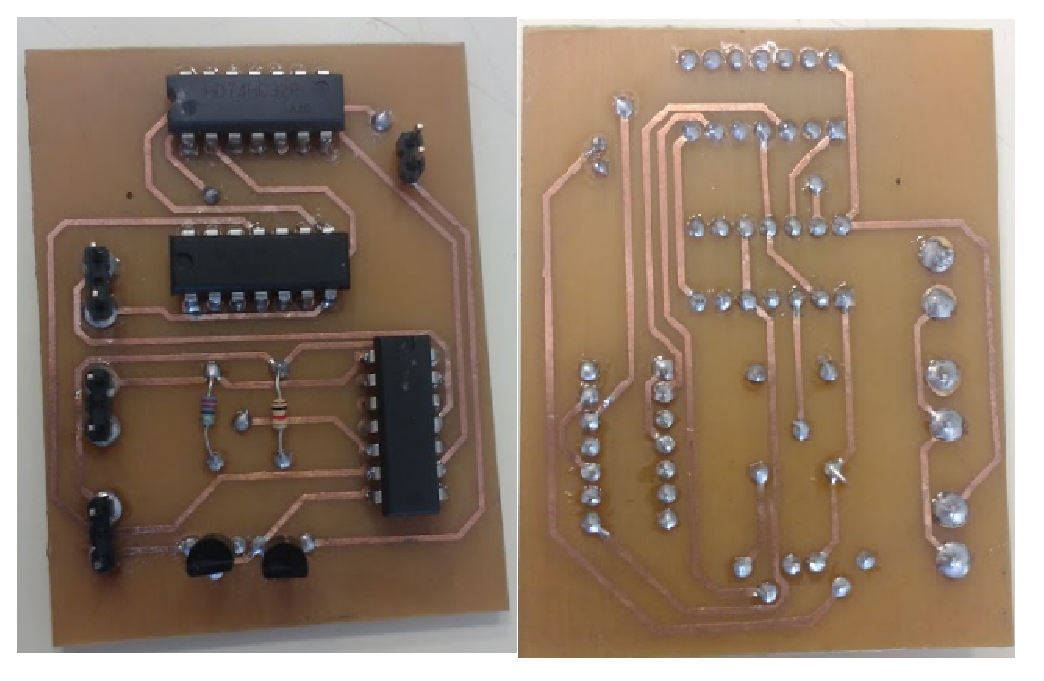
\includegraphics[scale=0.3]{../Exercise3/Assignment/images/TB}
\par\end{centering}
\caption{Printed Board}
\label{3_3}

\end{figure}

\subsection{\color{purple}Mealy State Machine Re-Implementation}

Finally, we were asked to re-implement the Moore State machine described
in the previous Subsections, into a Mealy State Machine. As we know,
Mealy Machines Outputs depend on states and inputs, different from
Moore that only depends on states. So the truth tables for the next
state, mantains its form and formula as the moore state machine, however,
the output truth table, and by consequence, its formula , change ash
shown on Table \ref{3_t_3}.

\begin{table}[H]
\begin{centering}
\begin{tabular}{|c|c|c|}
\hline 
State & W=0 & W=1\tabularnewline
\hline 
\hline 
00 & 00/0 & 01/1\tabularnewline
\hline 
01 & 00/0 & 10/0\tabularnewline
\hline 
10 & 00/0 & 10/0\tabularnewline
\hline 
\end{tabular}
\par\end{centering}
\caption{Mealy State Machine}
\label{3_t_4}
\end{table}

We can now easily see that in Table \ref{3_t_4}, states 01 and 10
are equal, so we can simplify those states into only one state. The
final Table is shown on Table \ref{3_t_5}.

\begin{table}[H]
\begin{centering}
\begin{tabular}{|c|c|c|}
\hline 
State & W=0 & W=1\tabularnewline
\hline 
\hline 
0 & 0/0 & 1/1\tabularnewline
\hline 
1 & 0/0 & 1/0\tabularnewline
\hline 
\end{tabular}
\par\end{centering}
\caption{Mealy Machine simplified}

\label{3_t_5}
\end{table}

\begin{table}[H]
\begin{centering}
\begin{tabular}{|c|c|c|}
\hline 
State & W & Output\tabularnewline
\hline 
\hline 
0 & 0 & 0\tabularnewline
\hline 
0 & 1 & 1\tabularnewline
\hline 
1 & 0 & 0\tabularnewline
\hline 
1 & 1 & 0\tabularnewline
\hline 
\end{tabular}
\par\end{centering}
\caption{Output Truth Table}

\label{3_t_3}
\end{table}

Finally, the formulas for the output and the next states are the following:

\[
Output=\bar{St}.W
\]

\[
State=W
\]

Implementing this would become someting like shown on Figure \ref{3_4}.

\begin{figure}[H]
\begin{centering}
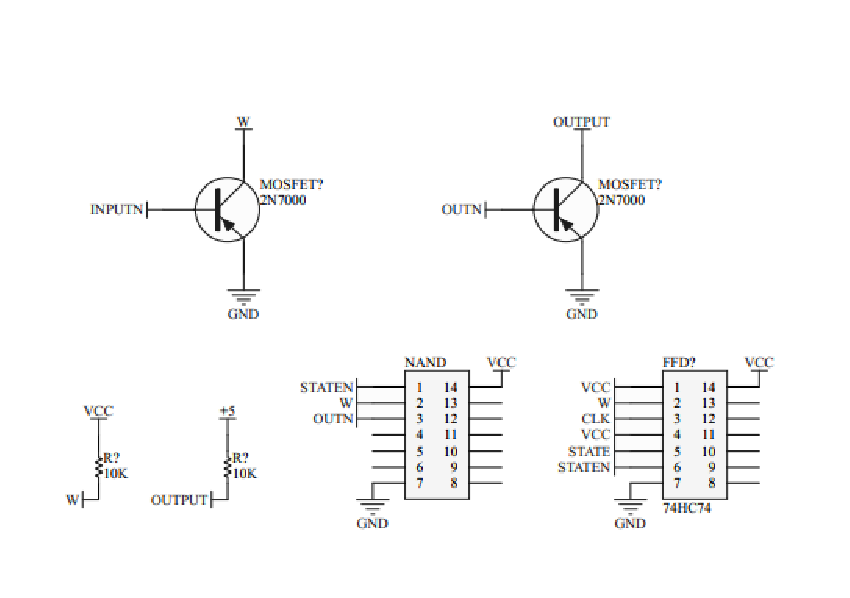
\includegraphics[scale=0.6]{../Exercise3/Assignment/images/Schematic2}
\par\end{centering}
\caption{Schematic Mealy Machine}
\label{3_4}

\end{figure}

We builded this schematic in a breadboard, as shon on Figure \ref{3_5}.

\begin{figure}[H]
\begin{centering}
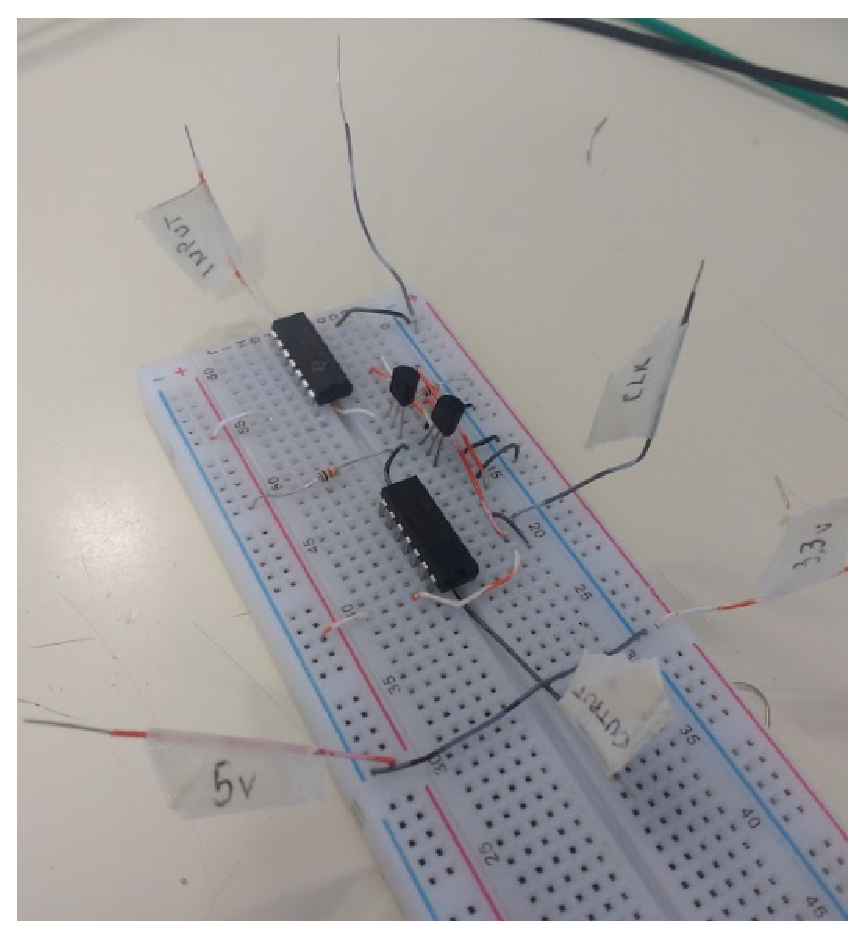
\includegraphics[scale=0.5]{../Exercise3/Assignment/images/mealy}
\par\end{centering}
\caption{Mealy Implementation}

\label{3_5}

\end{figure}

\subsection{\color{purple}Conclusions}

By analizing the behaviour of both circuits, how they behave in the
same test conditions, and comparing the amount of components used
in both PCBs, we conclude that in this case, Mealy's implementation
is more efficient because it utilizes less components and realizes
the same operation. However, we need to clarify that not always Mealy's
implementation is more efficient than Moore's, this depends on each
state machine to implement.
%\end{document}



%\newpage
\pagenumbering{roman}
\section{Appendix}

\begin{figure}[h!] %cambio la H por!
\begin{centering}
\includegraphics[scale=0.4]{../E4TP1/images/5}
\par\end{centering}
\caption{\color{cyan}Verilog implementation of Excercise 4}
\label{fig:figura4.6}
\end{figure}

\begin{figure}[h!]%cambio la H por!
\begin{centering}
\includegraphics[scale=0.4]{../E4TP1/images/6}
\par\end{centering}
\caption{\color{cyan}Terminal's output of Excercise 4}
\label{fig:figura4.7}
\end{figure}


%%% End document
\end{document}
